We measure the trigger efficiency by looking for trigger objects that match the candidate photon object in an appropriate data set because the trigger decisions are based on the existence of a single photon object in the event.
A trigger object is the four-momenta of an object reconstructed at the trigger level that is used for making trigger decisions. 
A trigger object is matched to the candidate when their angular separation  $\dR = \sqrt{\deta^2 + \dphi^2}$ is less than a certain threshold. 
For the photon candidate object, a line that connects the detector origin and the cluster position was used to define its direction because photons leave no tracks and do not bend in the magnetic field.

The trigger efficiency measurement is performed on the SingleMuon data set, exploiting events mostly from leptonic \ttbar\ (\Pe\Pgm) topology. 
Events with a candidate-quality photon without the pixel seed veto requirement and a muon object that passes the ``tight'' identifictaion requirement and matches the trigger object of the \texttt{HLT\_IsoMu24} or \texttt{HLT\_IsoTkMu24} triggers are used. 
The matching rate of the photon object and the trigger object is the trigger efficiency. 
Figure~\ref{fig:hlt_eff} shows the L1+HLT combined efficiency as a function of the photon \ET. 
It can be seen that the trigger is fully efficient for $\ET > 175\GeV$.

\begin{figure}[htbp]
  \centering
  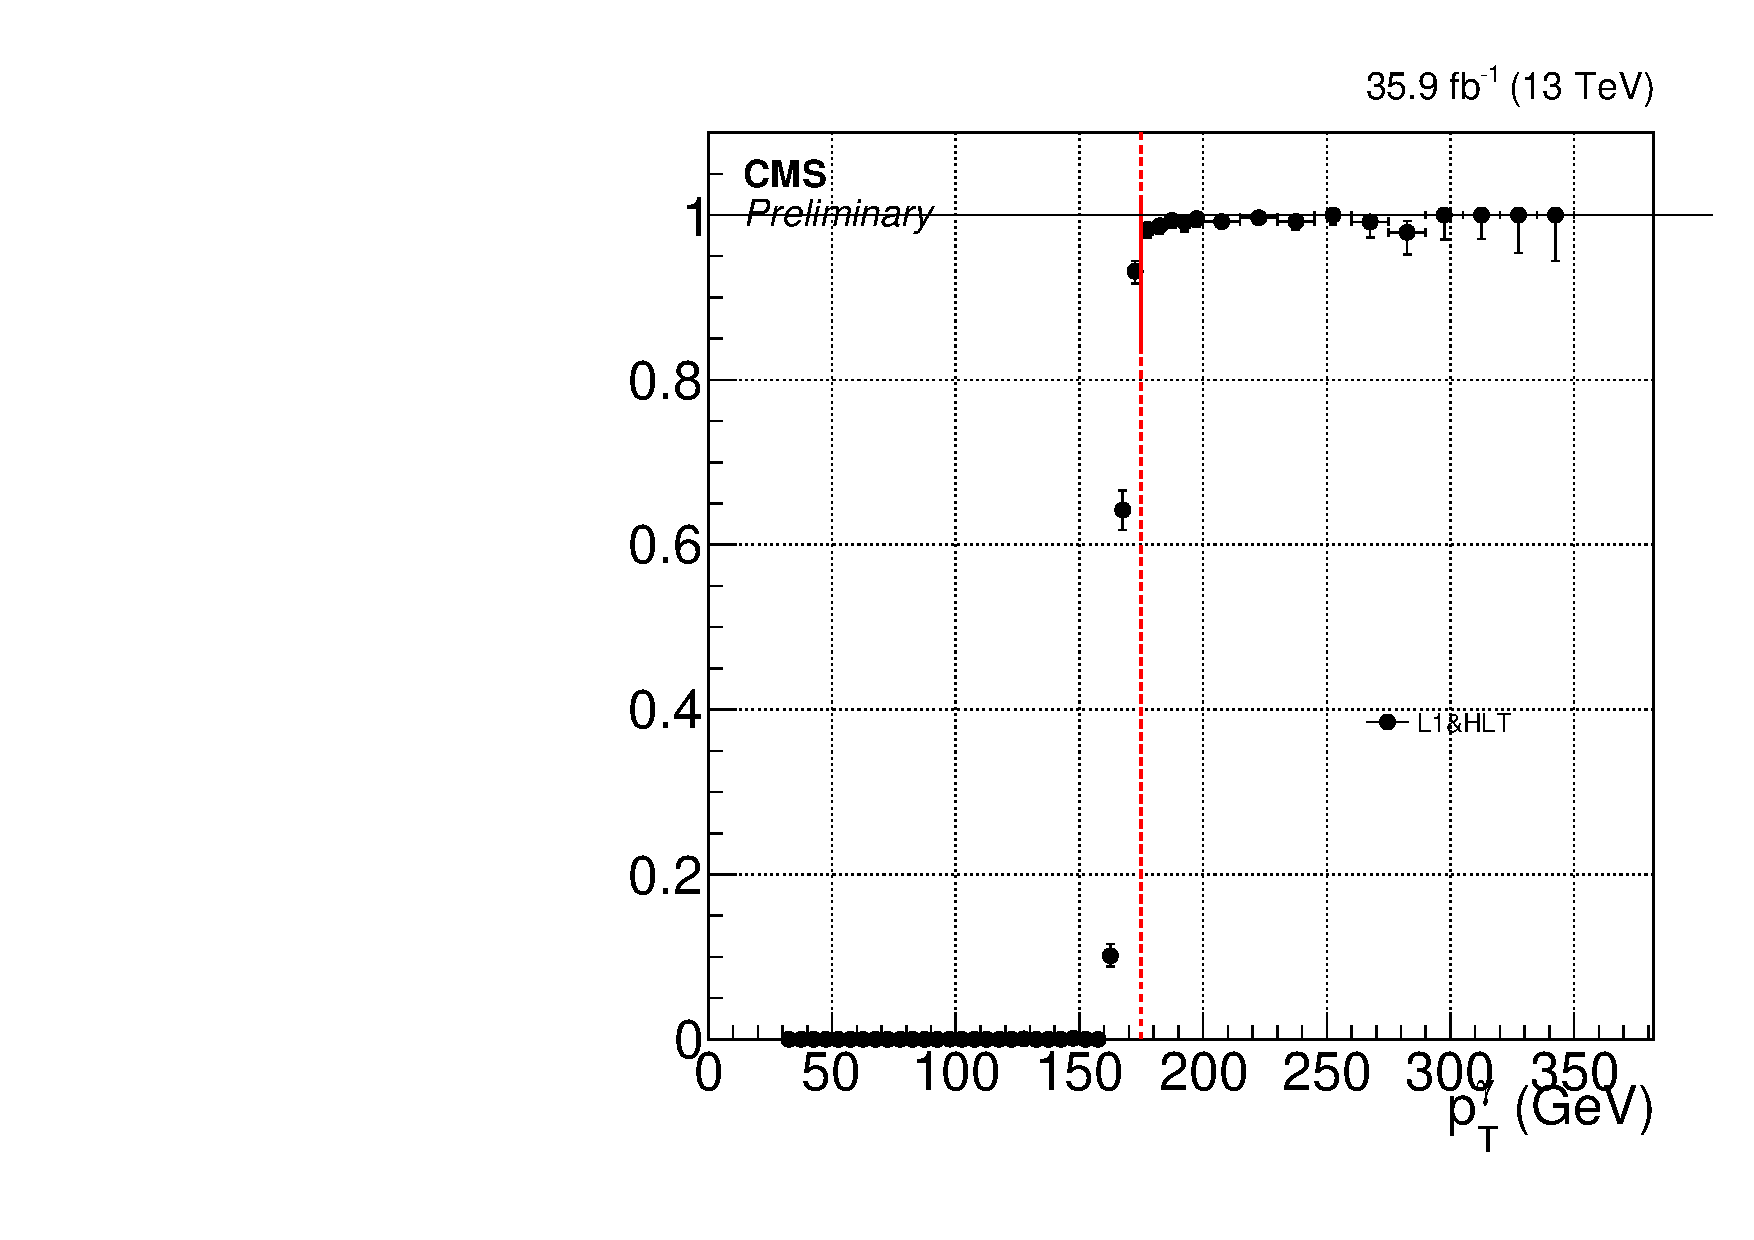
\includegraphics[width=0.48\textwidth]{Calibration/Figures/photon_elmu_sph165abs_ptzoom.pdf}
  \caption{
    The efficiency turn-on of the \texttt{HLT\_Photon165\_HE10} trigger for photons passing the candidate selection, measured using \Pgm\ + \egamma\ events from the SingleMuon data set. 
    Red vertical line corresponds to $\ET = 175\GeV.$
  }
  \label{fig:hlt_eff}
\end{figure}

For the first period of data taking, the \texttt{HLT\_Photon165\_HE10} trigger was seeded only by an isolated \egamma\ L1 trigger. 
This L1 seed becomes inefficient at high \ET\ due to a misconfiguration in the $H/E$ computation algorithm as indicated by the drop in efficiency at high-\ET\ shown in the left side of Figure~\ref{fig:l1_eff}. 
To mitigate the effect, in the later periods, the trigger was seeded by the logical \textbf{OR} of \texttt{SingleEG40} and \texttt{SingleJet} L1 triggers, combining multiple with various \pt\ thresholds.

Even with this addition, the measured trigger efficiency is not 100\% at the plateau, but it is flat with respect to \ET\ as shown on the right of Figure~\ref{fig:l1_eff}. 
In principle, the efficiency should be applied to all simulation-based background estimates whose normalization is fixed by theoretical calculation of the cross section.
However, the only simulation-based background processes with absolute normalization are those that contribute at $\mathcal{O}(1)$\%, with large systematic uncertainties. 
Therefore we deem the slight discrepancy of the trigger efficiency from unity as irrelevant.

\begin{figure}[htbp]
  \centering
  \resizebox{\textwidth}{!}{
    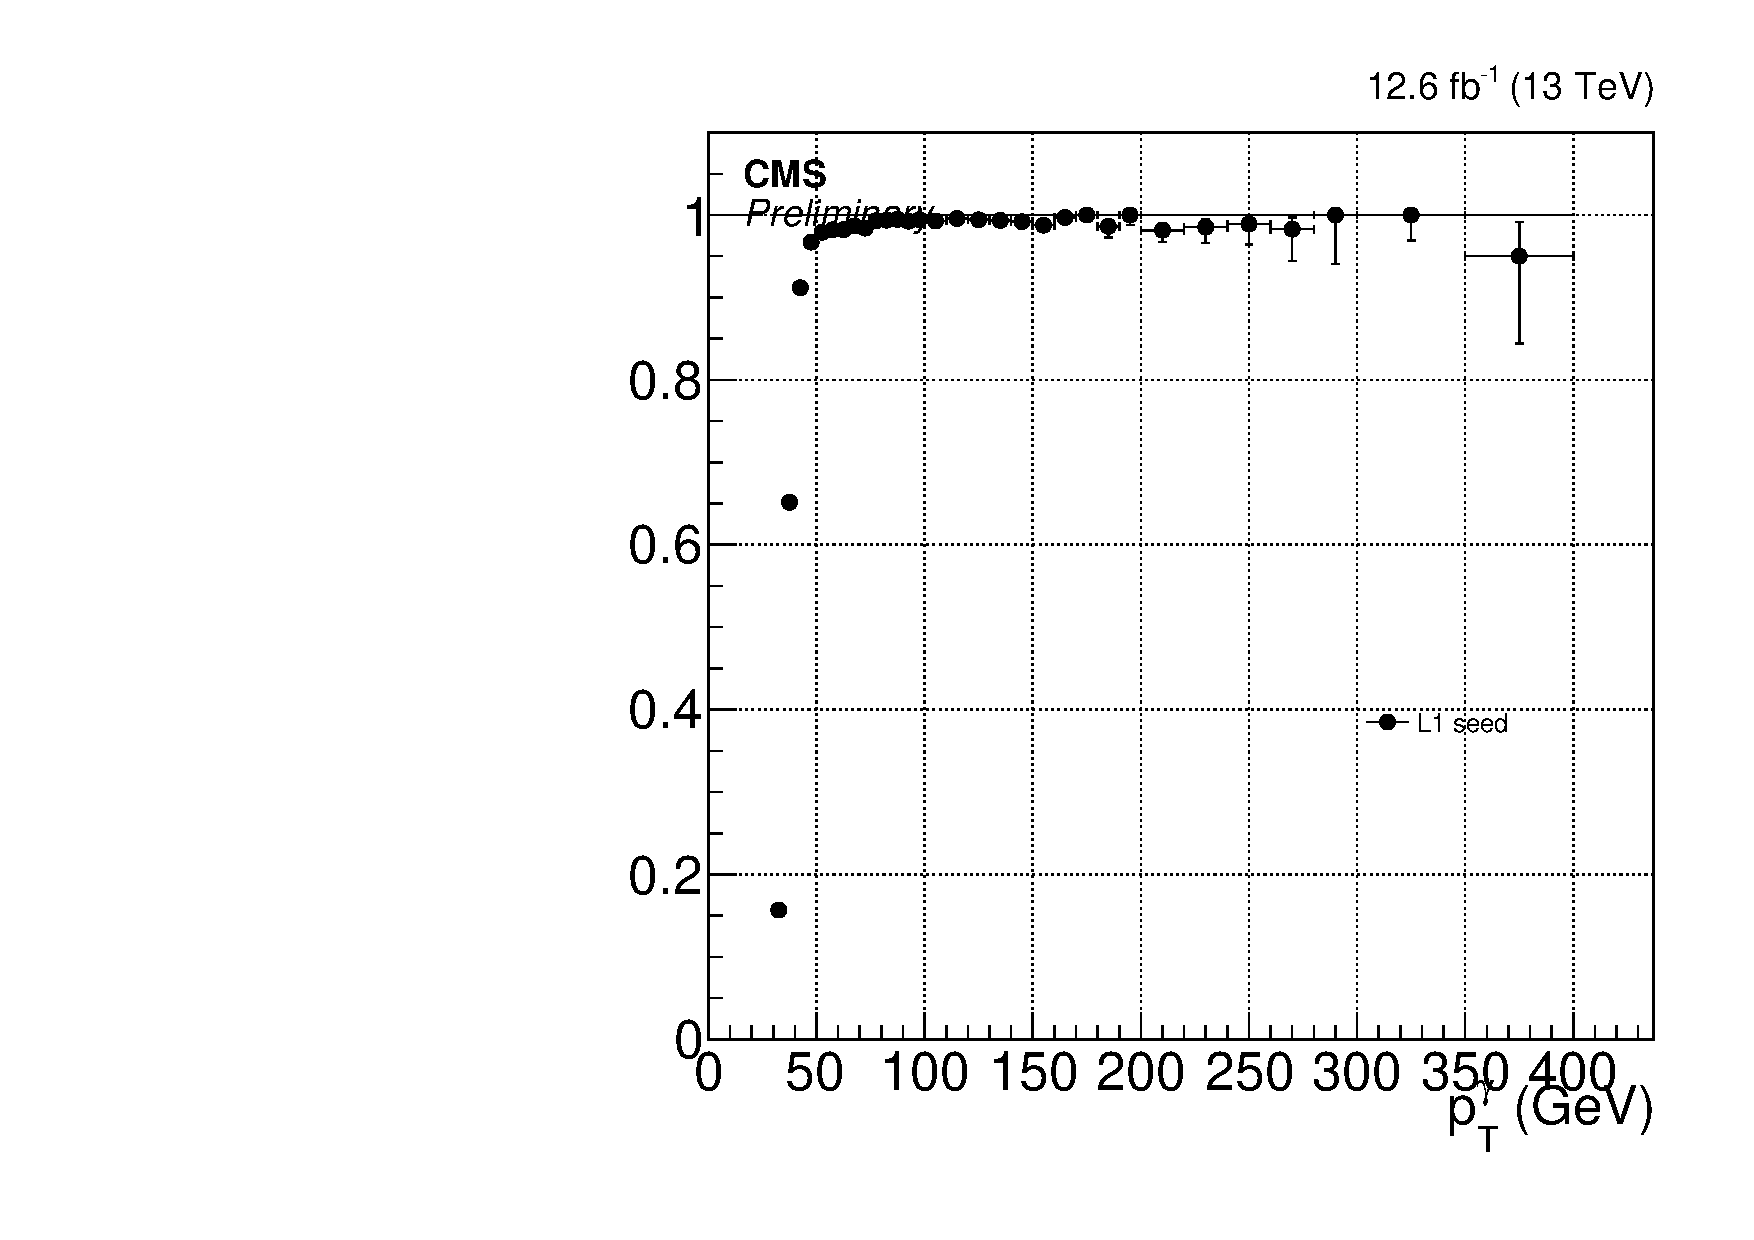
\includegraphics[]{Calibration/Figures/photon_elmuBCD_l1eg40_ptwide.pdf}
    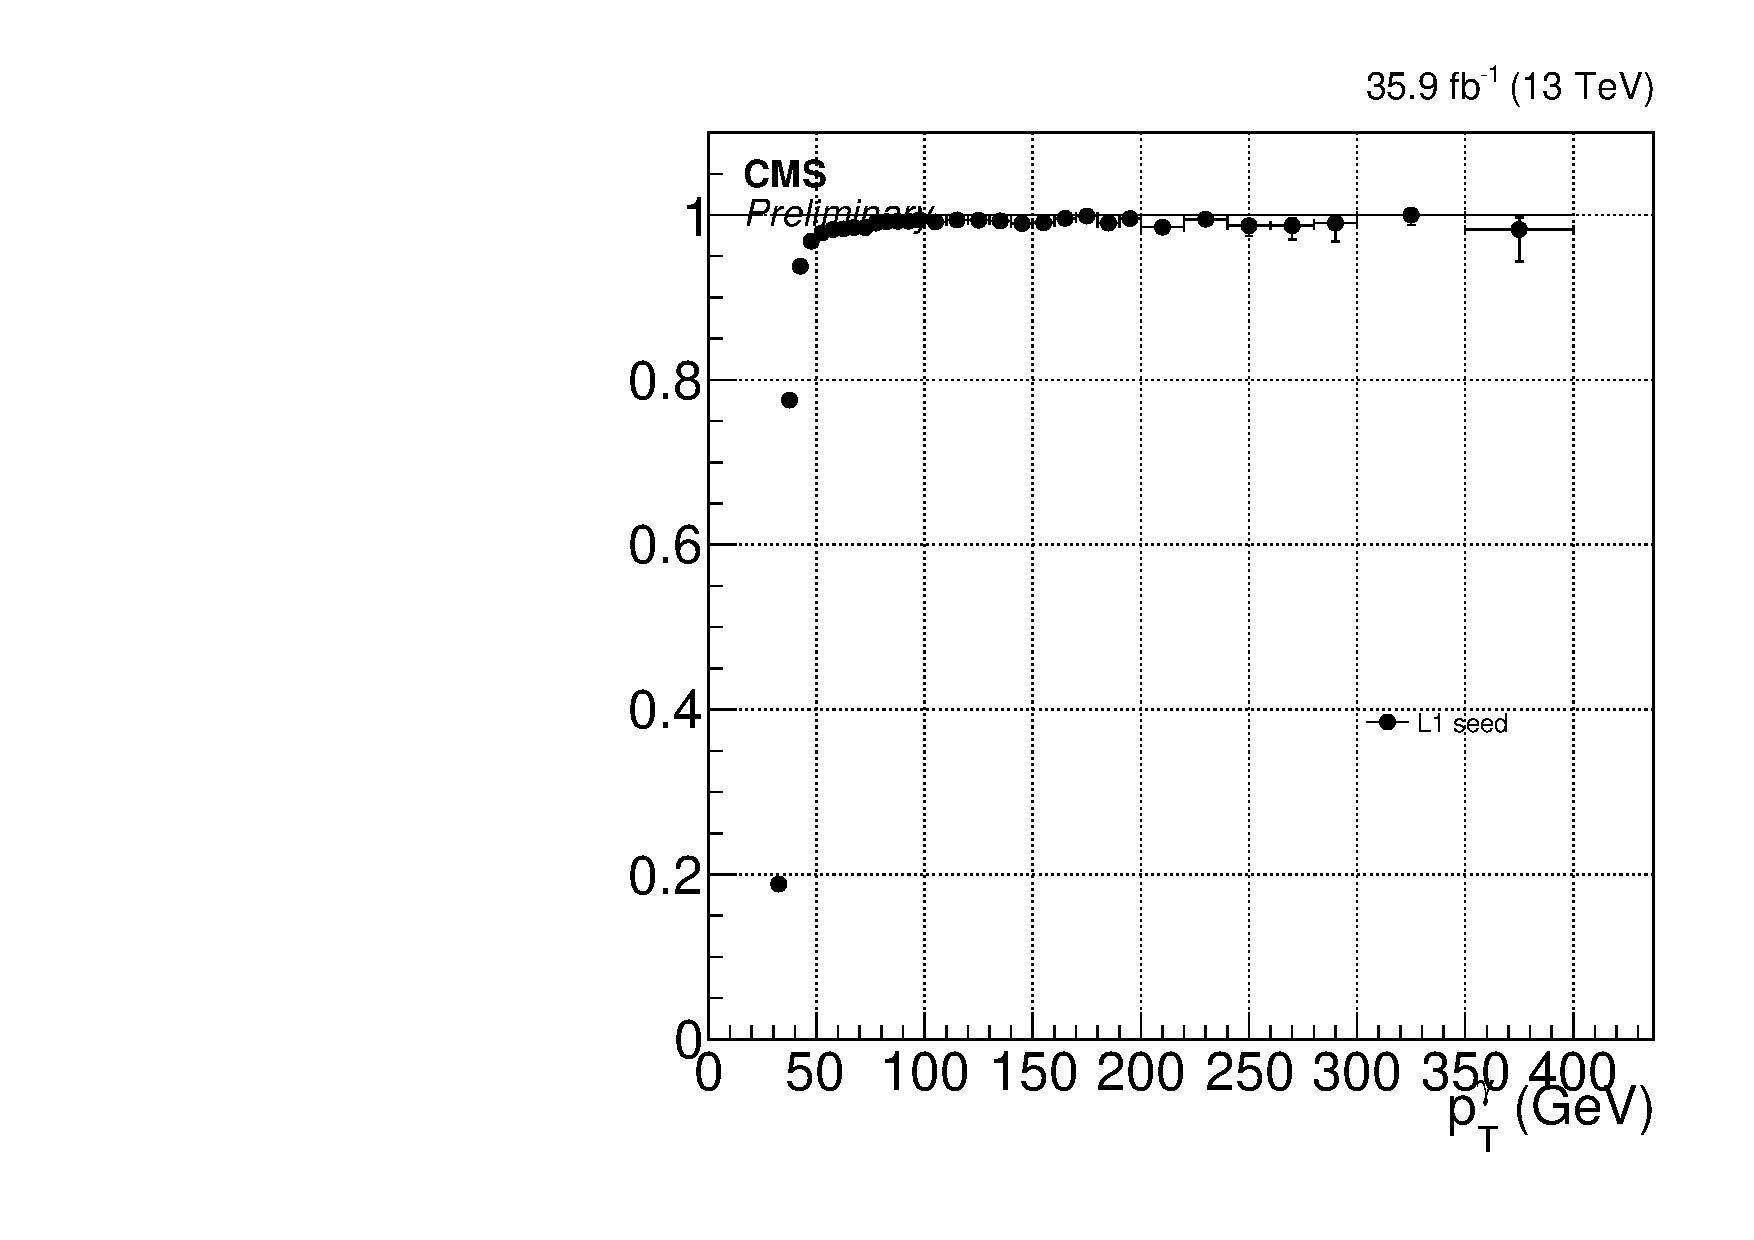
\includegraphics[]{Calibration/Figures/photon_elmu_l1all_ptwide.pdf}
  }
  \caption{
    The efficiency of the L1 seed for the signal trigger in periods B and C (left) and the full data set (right). The drop in efficiency at high-\ET\ in the earlier period is fixed by the addition of \texttt{SingleJet} L1 seeds during the remainder of data-taking. 
  }
  \label{fig:l1_eff}
\end{figure}
